\chapter{Fundamentação Teórica}
\label{chap:fund}

Neste capítulo serão abordados os principais conceitos de \emph{Deep Learning}, assim como as técnicas e algoritmos aplicados para auxiliar os profissionais de laboratório a realizarem hemogramas de uma forma eficiente. Além disso, serão apresentados os dados coletados de uma análise de sangue que dão subsídio para a geração de elementos de hemogramas.

\section{Exames Laboratoriais de Sangue}
\label{sec:conceito1}
Os exames laboratoriais de sangue, principalmente se tratando de hemogramas, são um tipo de exame simples, porém de extrema importância para a saúde humana. Através desses exames pode-se descobrir diversas informações sobre o organismo da pessoa examinada, inclusive detectar doenças e problemas antecipadamente, por exemplo, para diagnosticar anemia, deficiências nutricionais, parasitas no sangue, doenças virais e autoimunes. Também é possível identificar infecções, doenças como leucemia, diagnosticar efeitos de medicamentos e também o efeito de vários tipos de estresses sobre o corpo \cite{abcOfCbc, atlasDeHematologiaEAnalise}.

Um exame pode ser solicitado por um médico, ou a partir do interesse do próprio paciente, e realizado em um laboratório de análises clínicas, que será responsável por realizar a coleta, encaminhar para a análise específica e retornar o resultado. Todo esse processo é custoso em tempo de espera e também financeiramente, pois o maquinário para esse tipo de atividade constitui preço expressivo para aquisição e manutenção.

\subsection{Sangue}
O sangue é um elemento do corpo humano, que circula em estado líquido através de todo o sistema circulatório do organismo, sendo de importância para o funcionamento correto das células através da entrada e saída de substâncias que podem modificar a sua composição \cite{manualHematologia}.

Pode ser dividido em duas principais partes: o plasma (ou soro) e a parte celular. O plasma é a principal parte de transporte de substâncias pelo sistema, sendo este formado pela ingestão de água e alimentos. Também pode ser chamado de soro, sendo possível diferenciá-los pela presença ou não de anticoagulantes utilizados dependendo do tipo da análise buscada e da intenção da pesquisa \cite{interpretacaoHemograma}.

A segunda parte do sangue, que será objeto de estudo para este trabalho, é a parte celular que contém todas as células presentes no sangue e se classificam como glóbulos vermelhos, glóbulos brancos e plaquetas. Geralmente observa-se a presença de eritrócitos, vários tipos e classes de leucócitos e as plaquetas como um todo, que serão abordados um a um posteriormente \cite{atlasDeHematologiaEAnalise}.

\subsubsection{Glóbulos Vermelhos}
Os glóbulos vermelhos, também conhecidos como \emph{Red Blood Cells (RBC)}, são as hemácias presentes no sangue, também podem ser definidas em exames e registros médicos como eritrócitos. Essas células são pequenas e circulares, geralmente em formatos de discos e não possuem núcleo. Estão presentes em grande quantidade, possuindo uma vida útil de aproximadamente 120 dias até que o próprio sistema as elimine \cite{abcOfCbc}.

É indispensável, ao falar sobre a parte vermelha do sangue, citar a hemoglobina que é uma proteína presente nas hemácias e de extrema importância para o funcionamento do sistema, pois através dela é possível realizar o transporte de oxigênio e gás carbônico pelo sistema sanguíneo, permitindo as trocas gasosas necessárias \cite{manualHematologia}.

Percebe-se a presença dos glóbulos vermelhos na Figura \ref{fig:rbc}, onde estão em grande quantidade em comparação com as outras células. 

\begin{figure}[!htb]
	\centering
	\caption{Glóbulos Vermelhos (RBC)}
	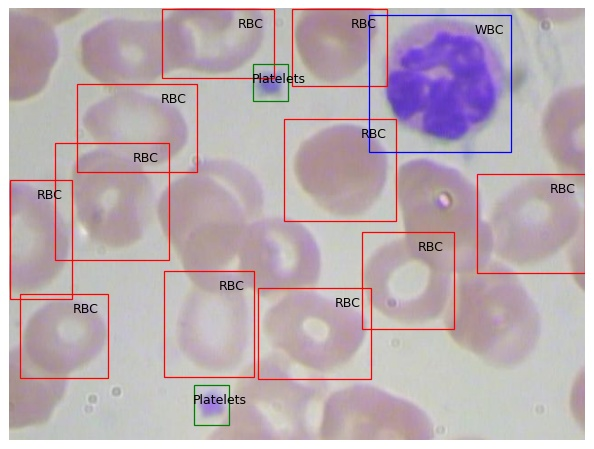
\includegraphics[width=0.40\textwidth]{img/rbc.jpg}
	\legend{Fonte: \citeonline{datasetBCCD}}
	\label{fig:rbc}
\end{figure}

A Figura \ref{fig:rbc} faz parte de um \emph{dataset}\footnote[1]{Um dataset é um grande conjunto de dados coletados.} específico de classificação de células sanguíneas, classificando em \emph{RBC (Red Blood Cells)} para glóbulos vermelhos, \emph{WBC (White Blood Cells)} para glóbulos brancos e \emph{Platelets} para plaquetas.
 
\subsubsection{Glóbulos Brancos}
Os glóbulos brancos, também conhecidos como \emph{White Blood Cells (WBC)}, são as células brancas do sangue, sendo responsáveis pela defesa do organismo contra as principais ameaças do corpo humano presentes no sistema sanguíneo. Através da fagocitose, que é um processo de englobamento de partículas sólidas pelas células, são realizadas ações de defesa contra a invasão de fragmentos estranhos. Os glóbulos brancos são criados na medula óssea e estão presentes em todo o sangue, também em grande quantidade \cite{abcOfCbc}.

Algumas células brancas podem ser encontradas na sua forma imatura, que ocorre quando o leucócito ainda não teve uma função definida pelo processo de maturação (promielócitos, mielócitos, metamielócitos). A maturação quando ocorre de forma adequada origina os seguintes tipos de leucócitos, cada qual com sua importância para o sistema de defesa do organismo \cite{manualHematologia}:

\begin{itemize}
	\item \textbf{Neutrófilos}: células brancas mais abundantes, capazes de entrar nos tecidos, onde conseguem realizar a defesa do organismo, fagocitando partículas estranhas. Essas células são conhecidas como neutrófilos segmentados, pois existe uma célula percursora, que é o bastão, ou também chamado de neutrófilos bastonetes, que possuem essa nomenclatura pois seu núcleo não está amadurecido, ou seja ainda são jovens, e geralmente são identificados quando há infecções em fase aguda. 
	\item \textbf{Eosinófilos}: células brancas responsáveis na defesa contra parasitas, geralmente estão presentes em grande quantidade no sangue durante reações alérgicas e infestações parasitárias.
	\item \textbf{Basófilos}: células brancas atuantes em respostas alérgicas e na coagulação do sangue. São capazes de liberar histamina, contribuindo para respostas alérgicas ao dilatar e permeabilizar os vasos sanguíneos e também liberam heparina que é capaz de prevenir a coagulação do sangue.
	\item \textbf{Monócitos}: células brancas capazes de entrar no tecido conjuntivo frouxo, onde conseguem se desenvolver em grandes células, com grande efeito fagocítico denominadas macrófagos, de forma a ingerir partículas estranhas ao organismo.
	\item \textbf{Linfócitos}: segundo tipo de célula branca mais abundante, são responsáveis e de extrema importância nas respostas imunes específicas do corpo humano, inclusive na produção de anticorpos.
\end{itemize}

Percebe-se também na Figura \ref{fig:wbc}, a presença dos glóbulos brancos entre os vermelhos, porém em menor quantidade.

\begin{figure}[!htb]
	\centering
	\caption{Glóbulos Brancos (WBC)}
	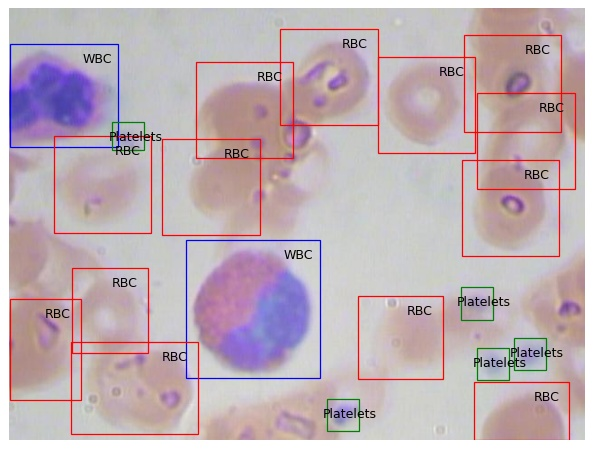
\includegraphics[width=0.40\textwidth]{img/wbc.jpg}
	\legend{Fonte: \citeonline{datasetBCCD}}
	\label{fig:wbc}
\end{figure}

Como visto na Figura \ref{fig:wbc}, embora existam várias classificações de glóbulos brancos, no \emph{dataset} onde foi coletada, não era objetivo de estudo realizar essa análise específica de cada célula.

\subsubsection{Plaquetas}
As plaquetas, também conhecidas e citadas como \emph{Platelets}, são os menores componentes do sangue e possuem grande responsabilidade na hemostasia, que é uma resposta fisiológica para a prevenção e interrupção de sangramentos e hemorragias, ou seja, elas atuam na manutenção dos vasos sanguíneos. As plaquetas são fragmentos do citoplasma de megacariócitos, ou seja, elas são produzidas na medula óssea como parte dessas células especializadas que irão se dividir posteriormente e gerar um grande número de plaquetas. Aproximadamente, para cada 1 megacariócito, pode-se produzir cerca de 4000 plaquetas \cite{abcOfCbc}.

Por serem fragmentos de uma célula, as plaquetas não possuem núcleo e são muito pequenas, com cerca de 1–3 µm\footnote[1]{1 micrômetro (µm) é equivalente à 0,001 milímetro.} de diâmetro, com a coloração azul-acinzentado. A vida útil das plaquetas dura em média de 9 a 12 dias, e elas são removidas pelo baço quando estão velhas ou danificadas \cite{abcOfCbc}.

Percebe-se também através da Figura \ref{fig:plaquetas}, a presença do último elemento visível abordado por este trabalho no \emph{dataset} utilizado como base. Nela é possível visualizar múltiplas plaquetas agrupadas em um dos cantos, além de outras no meio dos demais elementos do sangue.

\begin{figure}[!htb]
	\centering
	\caption{Plaquetas (Platelets)}
	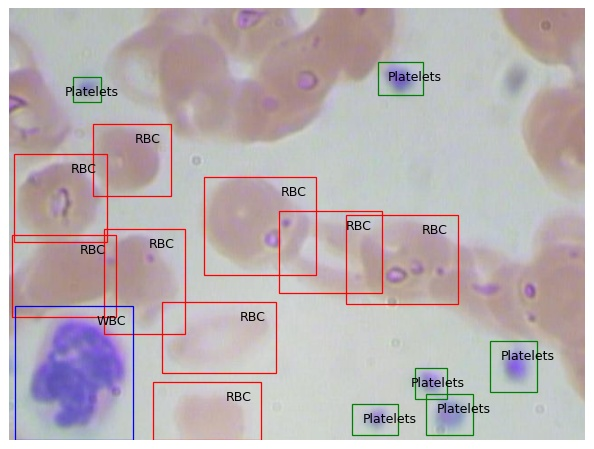
\includegraphics[width=0.40\textwidth]{img/plt.jpg}
	\legend{Fonte: \citeonline{datasetBCCD}}
	\label{fig:plaquetas}
\end{figure}

\subsection{Hemograma}
Um hemograma, também conhecido e citado como \emph{Complete Blood Count (CBC)}, é um exame bastante comum e muito utilizado, onde se realiza uma análise de sangue que envolve a contagem das diferentes células sanguíneas. A partir dos números obtidos através dessa contagem e com a comparação desse valor com as faixas de normalidade, é possível chegar a diversas conclusões sobre a saúde do paciente e até mesmo já identificar alguma doença ou problema \cite{manualHematologia, abcOfCbc}.

Um hemograma é geralmente realizado em duas principais etapas, sendo a primeira relacionada ao eritrograma que se refere à análise das células vermelhas, de forma a revelar até mesmo alguns tipos essenciais de alterações patológicas do sistema eritropoético, sendo o sistema responsável pela produção do material vermelho do sangue, como aumento na produção de glóbulos vermelhos e anemias. A segunda parte está relacionada com o leucograma, que corresponde à contagem global e específica dos leucócitos, a parte branca do sangue \cite{manualHematologia, abcOfCbc}.

\subsubsection{Eritrograma}
O objetivo do eritrograma ao realizar a análise da parte vermelha do sangue, é analisar alguns atributos-chave. Primeiramente é realizada a contagem geral dos eritrócitos adotando uma escala de milhões/mm³. A hemoglobina também é calculada e registrada em uma escala de g/dl \cite{interpretacaoHemograma, manualHematologia}.

Depois dessa contagem principal são calculados alguns índices, onde o primeiro deles apresenta o cálculo do volume corpuscular médio (VCM), sendo o volume médio das hemácias, calculado pelo quociente de um determinado volume de hemácias pelo número de células contidas no mesmo. Outro importante atributo é a hemoglobina corpuscular média (HCM), que semelhante ao VCM, apresenta o conteúdo médio da hemoglobina, calculado pelo quociente de conteúdo de hemoglobina em um determinado volume de hemácias pelo número de células contidas no mesmo volume \cite{interpretacaoHemograma, manualHematologia}.

Também temos outro índice que é a concentração de hemoglobina corpuscular média (CHCM), sendo a percentagem da hemoglobina em uma amostra de 100ml de hemácias. Por fim temos, a amplitude de distribuição dos glóbulos vermelhos, que em inglês significa \emph{Red Cell Distribution Width (RDW)}, que será responsável por avaliar a variação de tamanho entre as hemácias \cite{interpretacaoHemograma, manualHematologia}.

É possível visualizar a forma que esses índices do eritrograma estão presentes e são abordados em um hemograma real através da Figura \ref{fig:eritrograma}, assim como os seus respectivos valores de referência.

\begin{figure}[!htb]
	\centering
	\caption{Exemplo de Eritrograma e seus Atributos}
	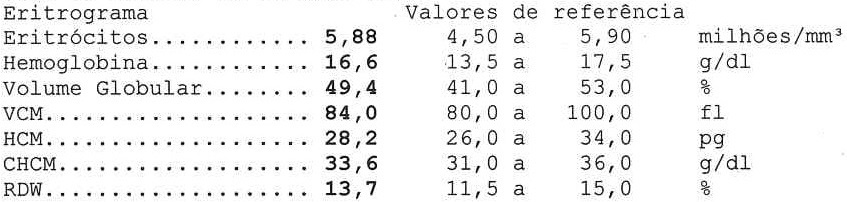
\includegraphics[width=0.80\textwidth]{img/eritrograma.jpg}
	\legend{Fonte: Elaborada pelo autor.}
	\label{fig:eritrograma}
\end{figure}
 
\subsubsection{Leucograma}
O objetivo do leucograma ao realizar a análise da parte branca do sangue, assim como no eritrograma, é analisar alguns atributos-chave, porém, diferente do processo anterior, essa etapa tem um foco muito maior na classificação e contagem de diferentes células brancas.

Primeiramente é feita uma contagem geral de leucócitos em mm³. Depois é realizada a contagem de forma a classificar cada tipo de leucócito presente, com neutrófilos, eosinófilos, basófilos, linfócitos, monócitos e também os granulócitos imaturos (promielócitos, mielócitos, metamielócitos). Por fim, também é calculado o número presente de plaquetas no sangue em mm³ \cite{interpretacaoHemograma, manualHematologia}.

É possível visualizar a maneira que os índices e classificações são abordados em um hemograma real através da Figura \ref{fig:leucograma}, assim como os seus respectivos valores de referência.

\begin{figure}[!htb]
	\centering
	\caption{Exemplo de Leucograma e seus Atributos}
	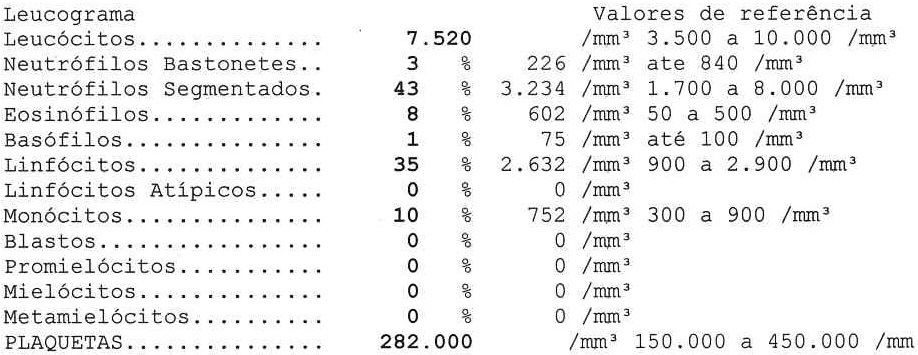
\includegraphics[width=0.80\textwidth]{img/leucograma.jpg}
	\legend{Fonte: Elaborada pelo autor.}
	\label{fig:leucograma}
\end{figure}

\section{Inteligência Artificial: \emph{Machine Learning e Deep Learning}}
\label{sec:conceito2}
A abordagem de \emph{Deep Learning}, que é objeto de estudo desse trabalho é uma das subáreas de \emph{Machine Learning}, que, por sua vez, é subárea de Inteligência Artificial, portanto antes de abordar cada um desses conceitos, quais suas diferenças e aplicações, se faz necessário introduzir o conceito de Inteligência Artificial.

A Inteligência Artificial é uma abordagem para a resolução de problemas de diversas naturezas de forma automatizada, ou seja, é uma maneira de se resolver problemas sem a necessidade de um humano ou usuário específico para esse trabalho. Essa área está recebendo muita atenção atualmente, buscando, cada vez mais, novas maneiras de automatizar tarefas do cotidiano. Essa abordagem está presente em diversos segmentos da indústria e atualmente também vem crescendo o uso nas residências para as mais diversas finalidades \cite{inteligenciaArtificial}.

O intuito dessa área é buscar formas de ensinar máquinas e computadores a serem capazes de ter uma inteligência cada vez mais semelhante aos seres humanos. Isso ocorre geralmente através do reconhecimento de padrões através de diversas técnicas, que permitem que os computadores sejam ensinados a analisar e interpretar dados, de forma semelhante ao que acontece no aprendizado de seres humanos. Porém, diferente de nós, as máquinas geralmente precisam de um volume massivo de dados para que sejam capazes de aprender algo básico \cite{IAAprendizadoMaquina}.

\subsection{Machine Learning}

A resolução de problemas através de ferramentas da computação é bastante comum e para isso se faz uso de algoritmos programados para finalidades específicas, porém não é em todos os problemas que se pode aplicar essa abordagem tradicional, porque nem sempre se sabe um caminho único de etapas a serem seguidas para chegar a uma resolução. Nesses casos, quando se sabe a entrada de dados e o resultado desejado, mas não os meios para se chegar nesse resultado, é possível utilizar um modelo de \emph{Machine Learning} para realizar a predição. É possível pensar da seguinte forma, na abordagem de algoritmos tradicionais de programação, possuímos os parâmetros necessários e conhecemos o método para assim chegar ao resultado, mas na aplicação de \emph{Machine Learning}, conhecemos os parâmetros e o resultado, porém o método será aprendido e apresentado pela própria máquina \cite{machineLearning}.

É possível fazer uma analogia entre um modelo de \emph{Machine Learning} e uma criança que aprende algo novo, onde todo modelo passa por três principais etapas: o pré-processamento dos dados, a fase de treinamento, e por fim o teste. Na fase de pré-processamento, os dados são analisados e adaptados para um melhor entendimento do modelo, retirando informações inúteis, alterando o formato para um mais adequado, entre outras práticas \cite{machineLearningPython}.

Logo após, o modelo de \emph{Machine Learning} deve ser treinado conforme o método desejado, antes de realizar a predição de qualquer valor ou resultado, onde o responsável pelo treinamento deverá fornecer um grande volume de dados, assim como os resultados esperados em cada um deles, além dos parâmetros e configurações necessárias para o treinamento. Dessa forma o modelo aprende a entender e interpretar os dados, tornando-se ser capaz de reproduzir esse método para prever o resultado de futuros dados \cite{machineLearningPython}.

Por fim, após o treinamento do modelo como um todo ocorre a fase de teste. Nesta fase, o modelo será testado e avaliado com base em algumas técnicas para medir o seu desempenho, calculando métricas como a acurácia, a precisão e a revocação. A acurácia indicará uma performance geral, ou seja, quantas classes o modelo classificou corretamente. A precisão dirá, dentre as classificações que o modelo classificou como positivo, quantas estão corretas. A revocação, também citada como \emph{recall}, apontará dentre todas as classificações que possuem positivo como valor esperado, quantas estão corretas. Além dessas métricas, também existe o F1-Score que realiza uma média harmônica entre precisão e \emph{recall} \cite{machineLearningTensorFlow}.

Para uma melhor visualização, e para realizar o cálculo das métricas citadas anteriormente, é comum a utilização de uma matriz de confusão, que descreve o número de acertos e erros relacionados com os verdadeiros ou falsos positivos e os verdadeiros ou falsos negativos, conforme observa-se na Figura \ref{fig:confusionMatrix} \cite{machineLearningTensorFlow}.

\begin{figure}[!htb]
	\centering
	\caption{Matriz de Confusão}
	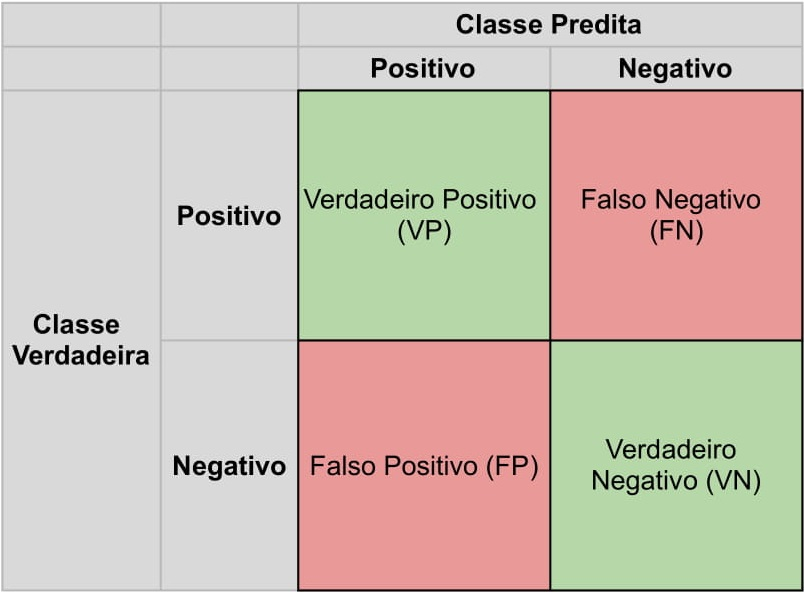
\includegraphics[width=0.50\textwidth]{img/confusionMatrix.jpg}
	\legend{Fonte: Elaborada pelo autor.}
	\label{fig:confusionMatrix}
\end{figure}

\subsubsection{Algoritmos Tradicionais}

Existem várias abordagens de \emph{Machine Learning}, que são divididas em duas metodologias diferentes: supervisionados ou não-supervisionados. No aprendizado supervisionado, sabe-se o resultado correto, ou seja, onde o modelo deverá chegar a partir dos dados obtidos, porém no aprendizado não-supervisionado, o modelo terá que lidar com dados não estruturados e sem um resultado claro \cite{machineLearningPython}.

Dentro do aprendizado supervisionado, encontra-se duas abordagens mais utilizadas, a regressão e a classificação. Os modelos de regressão serão responsáveis pela predição de valores reais, enquanto que os modelos de classificação serão responsáveis pela rotulação dos dados em determinadas classes \cite{machineLearningPython}.

Quando se trabalha com regressão de dados, é possível citar alguns exemplos de abordagens mais utilizadas \cite{machineLearningTensorFlow}.
\begin{itemize}
	\item \textbf{Linear Regression:} método mais clássico e simples para abordar regressão, onde é traçado uma reta através dos dados e então realizado a predição com base nessa reta. Possui variações como na \emph{Multiple Linear Regression} onde são usadas mais variáveis e também na \emph{Polynomial Linear Regression} onde a reta se tornará uma curva, utilizando variáveis com exponenciação, tornando o resultado mais assertivo.
	\item \textbf{Decision Tree:} árvore de decisão é uma técnica utilizada para prever valores através de critérios aprendidos pelo modelo. Esses critérios serão aprendidos através da divisão dos dados conhecidos em grupos semelhantes de forma a encontrar padrões em cada um dos grupos de dados.
	\item \textbf{Random Forest:} floresta aleatória é uma técnica utilizada de forma a combinar o poder de processamento de várias árvores de decisão diferentes, de forma a ter um trabalho mais minucioso e geralmente chegar em um resultado mais preciso.
\end{itemize}

Quando se trabalha com classificação de dados, é possível citar alguns exemplos de algoritmos mais utilizados \cite{machineLearningPython}.
\begin{itemize}
	\item \textbf{K-Nearest Neighbors (KNN):} o KNN é uma abordagem de um algoritmo que realizará a classificação com base na comparação de um dado com dados semelhantes a ele. É considerado uma abordagem \emph{lazy}, ou seja, preguiçosa, pois não apresenta um modelo inteligente, apenas armazena os dados e realiza comparações.
	\item \textbf{Decision Tree Classifier:} assim como na regressão, árvore de decisão é uma técnica utilizada para predizer classes para dados específicos a partir de uma série de critérios aprendidos pelo modelo. Esses critérios serão aprendidos através da divisão dos dados conhecidos em grupos semelhantes de forma a encontrar padrões que nesse caso seriam as classes necessárias para a interpretação em cada um dos grupos divididos de dados.
	\item \textbf{Random Forest Classifier:} assim como na regressão, floresta aleatória é uma técnica utilizada de forma a combinar o poder de processamento de várias árvores de decisão voltadas à classificação, buscando ter um trabalho mais minucioso e geralmente chegar em um resultado mais preciso.
\end{itemize}

Além desses algoritmos, é importante ressaltar uma abordagem diferente da convencional que são as redes neurais, que podem ser utilizadas tanto para regressão quanto para classificação. Esse tipo de abordagem se difere dos algoritmos tradicionais e será objeto de estudo desse trabalho.

\subsubsection{Redes Neurais}
\label{sec:redesneurais}

As redes neurais buscam uma abordagem bastante parecida com o cérebro humano, pois utilizam uma estrutura composta de \emph{perceptrons}, que são uma versão computadorizada de algo parecido com um neurônio humano. O \emph{perceptron} é capaz de receber \emph{inputs} (os dados de entrada) e produzir uma saída. O desempenho do uso de \emph{perceptrons} pode ser melhorado ao utilizar vários em conjunto formando uma rede, assim unindo o poder de processamento de cada um deles e chegando a um resultado mais assertivo em menor tempo. Para essa estrutura se dá o nome de rede neural artificial ou como é conhecida, \emph{Artificial Neural Network} (ANN) \cite{deepLearning, deepLearningTensorFlow}.

A Figura \ref{fig:perceptron} apresenta toda a estrutura de um \emph{perceptron}, onde o $x$ representa a informação repassada, o $w$ representa os pesos de cada informação, a letra $\Sigma$ o somatório, o $f$ a função de ativação e por fim o $y$ representa a saída.

\begin{figure}[!htb]
	\centering
	\caption{\emph{Perceptron}}
	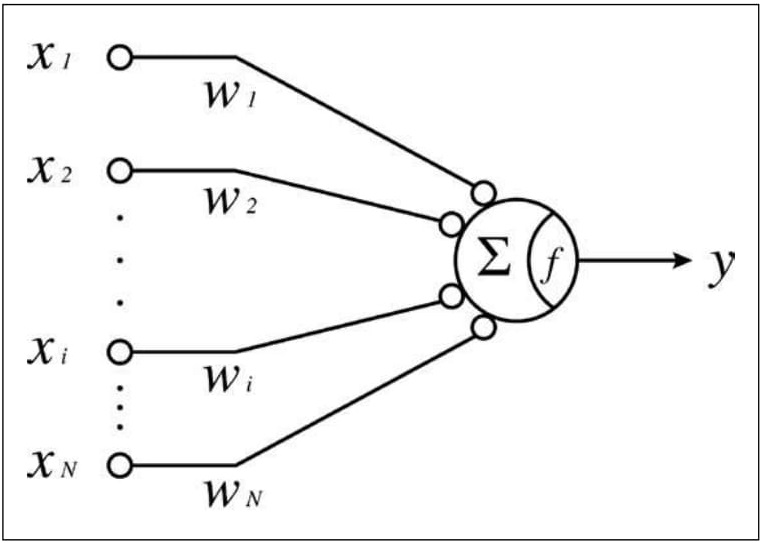
\includegraphics[width=0.50\textwidth]{img/perceptron.jpg}
	\legend{Fonte: \citeonline{deepLearning}}
	\label{fig:perceptron}
\end{figure}

Uma \emph{Artificial Neural Network} é uma estrutura formada por diversos neurônios, conhecidos como \emph{perceptrons}, organizados de forma a imitar o processamento de um cérebro humano. Sua estrutura é definida em diversas camadas, geralmente adotando uma camada de entrada, outra de saída e camadas intermediárias chamadas de ocultas que serão responsáveis pelo processamento na totalidade, onde cada uma delas pode conter um número variável de \emph{perceptrons} \cite{deepLearningTensorFlow}. Pode-se visualizar esta estrutura na Figura \ref{fig:neuralNetwork}, com a presença da camada de entrada, as camadas escondidas e por fim a camada de saída.

\begin{figure}[!htb]
	\centering
	\caption{Artificial Neural Network}
	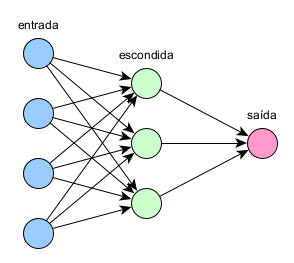
\includegraphics[width=0.40\textwidth]{img/neuralNetwork.png}
	\legend{Fonte: Elaborada pelo autor.}
	\label{fig:neuralNetwork}
\end{figure}

É importante ressaltar que além das informações repassadas de um \emph{perceptron} para o outro, existe outro fator importante para o seu funcionamento, sendo os pesos adotados. Os pesos são valores definidos para cada informação recebida pelo \emph{perceptron} e pode-se pensar no seu uso como um critério de prioridade entre uma informação e outra, que serão ajustados para alcançar o resultado desejado \cite{deepLearningTensorFlow}.

Dessa forma, uma ANN poderá aprender a realizar diversos tipos de tarefas, como classificação, por exemplo, através do uso de um algoritmo de \emph{backpropagation} que significa propagação regressiva, responsável por gerir a taxa de aprendizado do modelo, seguindo alguns passos \cite{deepLearningTensorFlow}.

Primeiramente, o algoritmo inicia a rede artificial com pesos aleatórios, entrando em modo de treino para realizar o aprendizado. Durante o treinamento, o algoritmo é capaz de realizar predições de resultados que serão comparados com os valores corretos, para saber se está obtendo sucesso ou não. O algoritmo de \emph{backpropagation} então calcula a diferença do resultado obtido com o real, e essa informação do erro é repassada para todas as camadas anteriores de forma a realizar um ajuste nos pesos e minimizar o erro \cite{deepLearningTensorFlow}.

Todo esse processo é realizado muitas vezes durante o treinamento, e só encerra quando os ajustes levam ao aumento do erro novamente, indicando que os pesos foram ajustados até o limite. Essa etapa de otimização dos pesos utilizados pela rede é muito importante, sendo essencial para o funcionamento da rede neural, pois através dela que é possível para o modelo aprender com os seus erros \cite{deepLearningTensorFlow}.

\subsection{Deep Learning}
Existem alguns casos que o \emph{Machine Learning} não é suficiente para o aprendizado a partir dos dados, pois o aprendizado acontece através de reconhecimento de padrões com base nos dados que não podem ser utilizados de qualquer forma, devem ser preparados e adaptados para cada modelo, ou seja, a máquina não é capaz de aprender por conta própria, pois precisa sempre de intervenção humana para o processamento dos dados. Logo, é preciso uma abordagem muito mais parecida com a forma de pensar dos seres humanos, como o \emph{Deep Learning} \cite{deepLearningPython, deepLearningTensorFlow}.

O \emph{Deep Learning} busca formas de aprofundar o conceito das redes neurais abordado na seção \ref{sec:redesneurais}, utilizando \emph{Deep Neural Networks (DNNs)}. As \emph{Deep Neural Networks (DNNs)}, ou Redes Neurais Profundas, são uma arquitetura de rede neural orientada ao \emph{Deep Learning}, ou seja, são muito mais complexas em seus modelos, com um número maior de neurônios, camadas ocultas em configurações mais complexas e conexões específicas entre os neurônios \cite{deepLearningTensorFlow}.

Com as possibilidades que as redes neurais profundas trouxeram, surgiram algumas variantes interessantes e focadas em um nicho específico, buscando se assemelhar ainda mais a natureza humana para realizar tarefas e criar inteligência. Algumas dessas variantes se aplicam a processamento de linguagem natural, como é o caso das RNNs abordadas na seção \ref{sec:rnn}, ou também abordam o reconhecimento e interpretação de imagens como é o caso das CNNs abordadas na seção \ref{sec:cnn} e é assunto de interesse para a continuidade deste trabalho.

\subsubsection{\emph{Recurrent Neural Networks (RNNs)}}
\label{sec:rnn}
As \emph{Recurrent Neural Networks}, ou Redes Neurais Recorrentes, são uma arquitetura de rede neural desenvolvida para a interpretação de dados temporais em sequência, ou seja, podem realizar predições de variáveis em relação ao tempo. Sua estrutura é desenvolvida para permitir conexões de feedback das informações repassadas, ou seja, possui \emph{loops} que permitem que as informações persistam, como se a rede fosse executada várias vezes. As RNNs são desenvolvidas para utilizar informações que possuem uma sequência fixa, como é o caso de informações que são atualizadas em decorrência do tempo \cite{deepLearningTensorFlow}.

\subsubsection{\emph{Convolutional Neural Networks (CNNs)}}
\label{sec:cnn}
As \emph{Convolutional Neural Networks}, ou Redes Neurais Convolucionais, são uma arquitetura de rede neural desenvolvida especificamente para o reconhecimento de imagens, com a capacidade de interpretar imagens dividindo-as em partes importantes. Essa rede trabalha inicialmente com 3 informações base, interpretando imagens como matrizes de 3 dimensões, sendo a altura, a largura e a cor \cite{deepLearningTensorFlow}.

As DNNs tradicionais funcionam bem para imagens pequenas, porém com um grande volume de dados, que nesse caso será cada pixel da imagem, o modelo teria muita dificuldade para aprender, logo nasceu a necessidade das CNNs. Para resolver esse problema, as CNNs foram desenvolvidas para usar camadas parcialmente conectadas e com grande reutilização dos pesos, dessa forma tem muito menos parâmetros à interpretar e passar adiante e consequentemente são mais rápidas para treinar, tendo menor risco de sobre-ajuste e necessitando de um volume menor de dados de treinamento \cite{deepLearningTensorFlow}.

Essa eficiência se deve também ao fato de que uma CNN, quando aprende a interpretar algum recurso ou elemento específico na imagem, torna-se capaz de identificar aquele elemento em qualquer lugar da imagem, diferentemente das DNNs que só aprendem a reconhecer um recurso em um local fixo. Isso mostra a capacidade das CNNs de serem mais generalistas em comparação com as DNNs \cite{deepLearningTensorFlow}.

Esse recurso pode ser encontrado dentro da camada convolucional, que está presente no início do processo e pode ser observada na Figura \ref{fig:cnn}. 

\begin{figure}[!htb]
	\centering
	\caption{Convolutional Neural Network}
	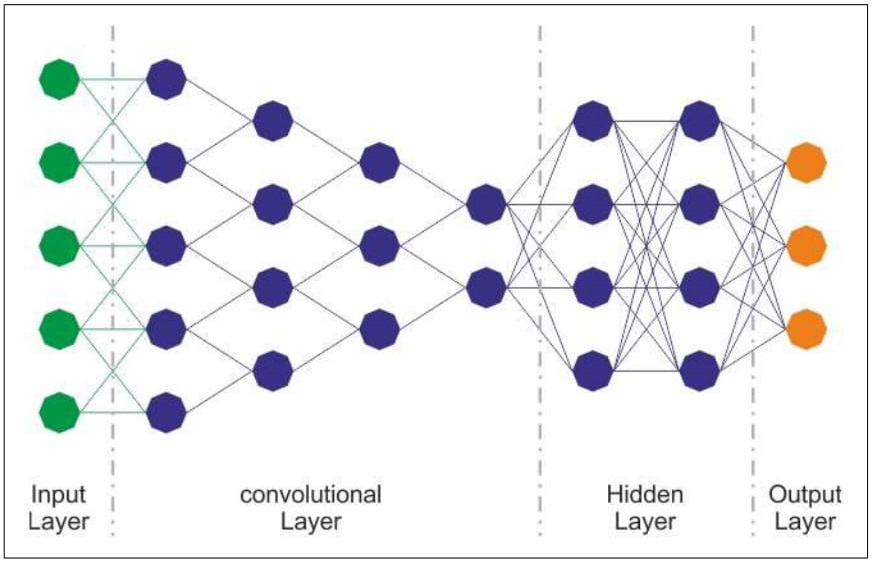
\includegraphics[width=0.60\textwidth]{img/cnn.jpg}
	\legend{Fonte: \citeonline{deepLearningTensorFlow}}
	\label{fig:cnn}
\end{figure}

\subsubsection{Bibliotecas e Recursos}
Para se trabalhar com \emph{Deep Learning} e suas principais arquiteturas e recursos, existem algumas bibliotecas disponíveis no mercado gratuitamente, as quais tendem a facilitar e orientar esse trabalho. Dessa forma, pode-se encontrar o Tensorflow e o Keras, sendo duas bibliotecas desenvolvidas em Python e C++, com a possibilidade de se trabalhar em conjunto e muito utilizadas pela comunidade de \emph{Deep Learning} em geral \cite{deepLearningTensorFlow}.

O Tensorflow é uma plataforma completa de código aberto para \emph{Machine Learning}, a qual considera uma grande variedade de tarefas com um foco nas redes neurais, porém suas funcionalidades também se estendem ao \emph{Deep Learning}. As APIs disponibilizadas do Tensorflow utilizam como base o próprio Keras para definir e treinar as redes neurais. Desenvolvido pelo Google desde 2011, em 2018 a equipe decidiu integrar o Keras na biblioteca principal do Tensorflow \cite{websiteTensorFlow}.

O Keras foi desenvolvido para permitir uma experimentação e prototipação rápida, com um principal foco nas redes neurais profundas. Promete ser fácil de utilizar, modular e ainda ser extensível. Possui vários recursos próprios, como a utilização de camadas, funções de perda, funções de ativação, entre outros. Além do foco em redes neurais profundas, possui módulos voltados a redes neurais convolucionais e recorrentes \cite{websiteKeras}.

O conjunto dessas duas bibliotecas para o trabalho com \emph{Machine Learning} e \emph{Deep Learning}, torna-se uma ferramenta extramente útil para este fim, possibilitando trabalhar com vários tipos de dados, como número, texto, áudio e também imagens.

Através da documentação do Tensorflow, é possível encontrar informações para desenvolver uma rede neural convolucional, por exemplo, onde existe toda a parte teórica e também a demonstração de um exemplo prático voltado a esse fim. Também é possível através dessa biblioteca e da sua documentação estar realizando a classificação de imagens com base em um \emph{dataset} de imagens \cite{websiteTensorFlow}.

Dentro do Tensorflow, também é possível estar trabalhando com diferentes módulos da biblioteca, nesse trabalho foi escolhido para uso o \emph{Object Detection}. Esse módulo é utilizado dentro dessa área para um objetivo bastante específico, que é a detecção de objetos contidos em uma imagem. Pode ser configurado para diversos usos, incluindo o caso desse trabalho, onde ao invés de detectar objetos físicos do dia a dia, o modelo é treinado para o reconhecimento de células em uma imagem e também para diferenciar uma célula das outras.

Com o \emph{Object Detection}, o tratamento das imagens e todo o processamento do modelo computacional se tornam tarefas mais fáceis de se trabalhar e também conta com outros vários recursos interessantes e úteis na hora do treinamento. Todo o algoritmo codificado para a realização do treinamento do modelo, contou com o apoio de funções do módulo do Tensorflow, \emph{Object Detection}.

\chapter{Estado da Arte da Área Pesquisada}
\label{chap:mapeamento}

O processo de pesquisa e seleção dos trabalhos relacionados, foi realizado com base em um mapeamento sistemático sobre as pesquisas com propostas para agilizar a identificação e interpretação de hemogramas. Este mapeamento resultou na identificação e seleção dos principais trabalhos de pesquisa no tema deste Projeto de Trabalho de Conclusão de Curso. Outro objetivo deste mapeamento sistemático foi verificar os métodos utilizados para a aplicação de \emph{Deep Learning} em imagens de amostras de sangue de maneira que possam ser obtidas informações para a geração automatizada de elementos de hemogramas.

\section{Mapeamento Sistemático da Literatura}

O mapeamento sistemático da literatura foi realizado com base na busca e levantamento de artigos, utilizando uma string de busca\footnote[1]{Uma string de busca é um conjunto de palavras-chave organizadas para auxiliar na pesquisa.} nas principais bibliotecas e repositórios de artigos. Esses artigos foram analisados e selecionados conforme a sua área de pesquisa e a sua temática, para inclusão nesse estudo. Para gerenciar o mapeamento sistemático foi utilizado a ferramenta Parsifal\footnote[2]{https://parsif.al/}, a qual auxilia na definição da string de busca, e permite salvar os artigos necessários e realizar a seleção.

As questões de pesquisas levantadas para isso foram, ``Como os algoritmos de \emph{Deep Learning} podem ser utilizados para a interpretação de exames?'' e ``Como realizar o tratamento de imagens para reconhecimento por modelos de \emph{Deep Learning}?''. A partir dessas questões foram extraídas palavras e termos para o direcionamento da pesquisa. É possível visualizar estas palavras com seus sinônimos na Tabela \ref{tbl:palavrasChave}.

\begin{table}[!htb]
	\centering
	\caption{Palavras-Chave e Sinônimos}
	\label{tbl:palavrasChave}
	\begin{tabular}{|c|c|}
		\hline
		\textbf{Palavra-Chave} & \textbf{Sinônimos}                                        \\ \hline
		Blood Analysis         & Blood Sample                                               \\ \hline
		Classification         & Interpretation, Recognition                                \\ \hline
		Deep Learning          & Artificial Intelligence, Computer Vision, Machine Learning \\ \hline
	\end{tabular}
	\vspace{6pt}
	\legend{Fonte: Elaborada pelo autor.}
\end{table}

Na Tabela \ref{tbl:basesDeDados}, são listadas as bases de dados onde os artigos foram coletados, a quantidade de cada um deles e a string de busca utilizada na seleção. A mesma string de busca foi utilizada nas três bases de dados, e os artigos encontrados foram dos últimos 5 anos (2016-2021).

\begin{table}[!htb]
	\centering
	\caption{Bases de Dados e Número de Artigos Selecionados}
	\label{tbl:basesDeDados}
	\begin{tabular}{|c|c|c|}
		\hline
		\textbf{Base de Dados}                & \textbf{Artigos}     & \textbf{String de Busca}                                                                                     \\ \hline
		\multirow{2}{*}{ACM Digital Library}  & \multirow{2}{*}{37}  & \multirow{6}{*}{\begin{tabular}[c]{@{}c@{}}(``classification'' OR ``interpretation'' OR ``recognition'') AND \\  (``deep learning'' OR ``artificial intelligence'' \\ OR ``computer vision'' OR ``machine learning'') AND\\  (``blood analysis'' OR ``blood sample'')\end{tabular}} \\
		                                      &                      &                                                                                                              \\ \cline{1-2}
		\multirow{2}{*}{IEEE Digital Library} & \multirow{2}{*}{13}  &                                                                                                              \\
		                                      &                      &                                                                                                              \\ \cline{1-2}
		\multirow{2}{*}{Scopus}               & \multirow{2}{*}{114} &                                                                                                              \\
		                                      &                      &                                                                                                              \\ \hline
	\end{tabular}
	\vspace{6pt}
	\legend{Fonte: Elaborada pelo autor.}
\end{table}

\subsection{Critérios de Exclusão}

Os artigos coletados na pesquisa através da string de busca, passaram por critérios de exclusão por não se adequarem a esta pesquisa, esses critérios podem ser observados na Tabela \ref{tbl:exclusao}. 

\begin{table}[!htb]
	\centering
	\caption{Critérios de Exclusão}
	\label{tbl:exclusao}
	\begin{tabular}{|c|c|}
		\hline
		\textbf{Critério de Exclusão}                    & \textbf{Nº de Artigos Recusados} \\ \hline
		O estudo não faz parte da área de pesquisa       & 101                               \\ \hline
		O estudo apresenta resultados fora da computação & 29                                \\ \hline
		O estudo não é um estudo primário               & 6                                 \\ \hline
		O estudo é duplicado                              & 16                                \\ \hline
	\end{tabular}
	\vspace{6pt}
	\legend{Fonte: Elaborada pelo autor.}
\end{table}

A seleção iniciou com 164 artigos no total das três bases de dados pesquisadas. Com a aplicação dos critérios de exclusão, observa-se um resultante de apenas 12 artigos. Isso ocorreu, pois, 101 artigos foram eliminados no critério ``O estudo não faz parte da área de pesquisa'', que significa que esses artigos tinham alguma relação, porém eram voltados a outras áreas. Outros 29 artigos foram eliminados no critério ``O estudo apresenta resultados fora da computação'', que significa serem da área de pesquisa, porém com resultados e métodos sem conexão com a computação. Foram também encontrados 6 artigos, que foram eliminados no critério ``O estudo não é um estudo primário'', o que indica que o artigo pode ser uma revisão sistemática da literatura ou semelhante. Por fim, foram eliminados outros 16 artigos por serem duplicados.

\subsection{Critérios de Inclusão}

Os seguintes critérios de inclusão foram definidos:
\begin{itemize}
	\item Nova tecnologia para análise de hemogramas;
	\item Processo, método ou técnica para contagem de células sanguíneas;
	\item Sistema para elaboração de hemogramas utilizando Deep Learning;
\end{itemize}

Na Tabela \ref{tbl:mapeamento}, é possível visualizar todos os 12 artigos selecionados com base nos critérios de inclusão, uma vez que todos eles se enquadram em pelo menos um deles.

\begin{table}[!htb]
	\centering
	\caption{Artigos Selecionados}
	\label{tbl:mapeamento}
	\begin{tabular}{|c|l|l|}
		\hline
		\textbf{ID} & \multicolumn{1}{c|}{\textbf{Título do Artigo}} & \multicolumn{1}{c|}{\textbf{Autores}}                     \\ \hline
		A1          & \begin{tabular}[c]{@{}l@{}}Analyzing microscopic images of           \\ peripheral blood smear \\ using deep learning\end{tabular} & \begin{tabular}[c]{@{}l@{}}Mundhra, D. and Cheluvaraju, B. \\ and Rampure, J. and Rai Dastidar, T.\end{tabular} \\ \hline
		A2          & \begin{tabular}[c]{@{}l@{}}Automatic detection and classification    \\ of leukocytes using \\ convolutional neural networks\end{tabular} & \begin{tabular}[c]{@{}l@{}}Zhao, J. and Zhang, M. \\ and Zhou, Z. and Chu, J. and Cao, F.\end{tabular} \\ \hline
		A3          & \begin{tabular}[c]{@{}l@{}}Automatic white blood cell classification \\ using pre-trained deep learning models: \\ ResNet and Inception\end{tabular} & \begin{tabular}[c]{@{}l@{}}Habibzadeh, M. and Jannesari, M. \\ and Rezaei, Z. and Baharvand, H. \\ and Totonchi, M.\end{tabular} \\ \hline
		A4          & \begin{tabular}[c]{@{}l@{}}Classification of Human White             \\ Blood Cells Using Machine Learning \\ for Stain-Free Imaging \\ Flow Cytometry\end{tabular} & \begin{tabular}[c]{@{}l@{}}Lippeveld, M. and Knill, C. and \\ Ladlow, E. and \\ Fuller, A. and Michaelis, L.J. and \\ Saeys, Y. and Filby, A. and Peralta, D.\end{tabular} \\ \hline
		A5          & \begin{tabular}[c]{@{}l@{}}Blood cell classification using the hough \\ transform and \\ convolutional neural networks\end{tabular} & \begin{tabular}[c]{@{}l@{}}Molina-Cabello, M.A. and López-Rubio, E. \\ and Luque-Baena, R.M. and \\ Rodríguez-Espinosa, M.J. and \\ Thurnhofer-Hemsi, K.\end{tabular} \\ \hline
		A6          & \begin{tabular}[c]{@{}l@{}}White Blood Cells Image Classification    \\ Using Deep Learning with \\ Canonical Correlation Analysis\end{tabular} & Patil, A.M. and Patil, M.D. and Birajdar, G.K. \\ \hline
		A7          & \begin{tabular}[c]{@{}l@{}}Image processing and machine learning     \\ in the morphological analysis \\ of blood cells\end{tabular} & \begin{tabular}[c]{@{}l@{}}Rodellar, J. and Alférez, S. and Acevedo, A. \\ and Molina, A. and Merino, A.\end{tabular} \\ \hline
		A8          & \begin{tabular}[c]{@{}l@{}}Improving blood cells classification in   \\ peripheral blood smears using \\ enhanced incremental training\end{tabular} & Al-qudah, R. and Suen, C.Y. \\ \hline
		A9          & \begin{tabular}[c]{@{}l@{}}Corruption-Robust Enhancement of          \\ Deep Neural Networks\\ for Classification of Peripheral \\ Blood Smear Images\end{tabular} & \begin{tabular}[c]{@{}l@{}}Zhang, S. and Ni, Q. and Li, B. and \\ Jiang, S. and \\ Cai, W. and Chen, H. and Luo, L.\end{tabular} \\ \hline
		A10         & \begin{tabular}[c]{@{}l@{}}Convolutional neural network and decision \\ support in medical imaging:\\ Case study of the recognition of \\ blood cell subtypes\end{tabular} & Diouf, D. and Seck, D. and Diop, M. and Ba, A. \\ \hline
		A11         & \begin{tabular}[c]{@{}l@{}}Combining Convolutional Neural Network    \\ With Recursive Neural Network \\ for Blood Cell Image Classification\end{tabular} & \begin{tabular}[c]{@{}l@{}}Liang, G. and Hong, H. and Xie, W. and\\ Zheng, L.\end{tabular} \\ \hline
		A12         & \begin{tabular}[c]{@{}l@{}}Blood diseases detection using            \\ classical machine learning algorithms\end{tabular} & Alsheref, F.K. and Gomaa, W.H. \\ \hline
	\end{tabular}
	\vspace{6pt}
	\legend{Fonte: Elaborada pelo autor.}
\end{table}

Todos os artigos selecionados estão relacionados à recursos para auxiliar na interpretação de exames de sangue utilizando conceitos de \emph{Deep Learning} e \emph{Machine Learning}.

\section{Análise dos trabalhos selecionados}

Por fim, com os artigos selecionados e classificados, foi realizada a extração dos dados desses trabalhos, sendo essa a última etapa desse mapeamento sistemático da literatura. É possível perceber que os algoritmos e abordagens mais utilizados são técnicas de \emph{Deep Learning}, como, por exemplo, o uso de \emph{Convolutional Neural Network (CNN)} (A1, A2, A3, A4, A5, A6, A8, A9, A10, A11) e de \emph{Recurrent Neural Network (RNN)} (A6, A11), sendo abordagens de redes neurais para a classificação das células sanguíneas.

Outros trabalhos utilizam de algoritmos de \emph{Machine Learning} tradicionais para a classificação, como por exemplo, o uso de \emph{Random Forest} ou \emph{Decision Trees}  (A2, A4, A7), sendo estruturas de árvores de decisão. Também foram encontrados estudos recorrendo a \emph{Support Vector Machine (SVM)} (A7) que utilizam vetores de suporte e por fim \emph{K-Means e K-Nearest Neighbors (KNN)} (A12), que fazem a classificação considerando os vizinhos mais próximos.

\chapter{Metodologia}
\label{chap:metodologia}
% Dataset
% Preparação dos dados
% Modelagem do problema
% Avaliação
% Implantação (protótipo)

Para a realização deste trabalho, muitos passos foram seguidos e desenvolvidos. Desde o estudo com o \emph{dataset} escolhido, a preparação dos recursos necessários como as bibliotecas e o ambiente, até o treinamento do modelo e por fim o desenvolvimento do protótipo final. Neste capítulo, todas as etapas realizadas no projeto serão descritas em detalhes, para facilitar a compreensão dos passos executados para alcançar objetivos propostos.

\section{\emph{Dataset}}
Para a realização de trabalhos na área de inteligência artificial, a escolha do \emph{dataset} é uma tarefa de extrema importância e deve ser feita com bastante estudo, pois impacta em todo o andamento dos processos seguintes. Durante a busca pelo \emph{dataset}, alguns candidatos surgiram, mas a escolha que se mostrou mais adequada foi de utilizar o BCCD Dataset. \cite{datasetBCCD}

A escolha por esse \emph{dataset} se deu, primeiramente, pelo maior número de trabalhos referenciando esta fonte. Também observou-se que em comparação com os outros \emph{datasets} disponíveis na literatura, esse é o mais completo e aprofundado para esta área de pesquisa. Outro fator decisivo, foi a sua quantidade de imagens, que além de estarem em uma quantidade considerável para o uso, também apresentam boa qualidade para a interpretação visual e para o treinamento de modelos de \emph{Deep Learning}.

O \emph{dataset} apresenta três categorias de detecção WBC (\emph{White Blood Cell}) para as células brancas, RBC (\emph{Red Blood Cell}) para as células vermelhas e também as \emph{Platelets}, para as plaquetas. Os arquivos estão separados em diretórios diferentes, onde em uma das pastas temos todo o conjunto de imagens, e em outra pasta temos as coordenadas de cada uma das células nas imagens, em formato XML.

Com o \emph{dataset} em mãos, foi iniciado o estudo e aprofundamento de seu conteúdo, considerando os seus recursos e também suas limitações. Inicialmente foi possível perceber que uma das limitações do \emph{dataset} é que nem todas as células nas imagens possuem coordenadas mapeadas. Grande parte apresenta o mapeamento correto, porém existem células que não apresentam nenhuma coordenada, e isso é uma falha do \emph{dataset} que pode afetar o treinamento do modelo.

Outra limitação também observada nesse \emph{dataset}, é a falta de classificação das células brancas. O \emph{dataset} se preocupa apenas em localizar as células na imagem e categorizar em brancas, vermelhas e plaquetas. Porém, para se elaborar um hemograma completo, isso não é suficiente. Para a elaboração do hemograma, é necessário além de realizar a contagem das células brancas, também realizar a sua classificação (Neutrófilos, Basófilos, Eosinófilos, Linfócitos, Monócitos, entre outros), para através disso se ter um diagnóstico mais concreto a respeito do paciente. A introdução da detecção das classes para as células brancas ficará listada como possível trabalho futuro.

Com a obtenção do \emph{dataset}, iniciou-se a fase de adaptação do conjunto de imagens para a detecção pelo modelo. No repositório, além das imagens, também estão contidos alguns programas \emph{Python}, que servem para o tratamento dos dados como uma forma de demonstrar possíveis usos para o \emph{dataset}. Como por exemplo, um programa capaz de fazer o contorno das células para uma pré-visualização dos dados. Porém, como este trabalho envolve a aplicação de um modelo computacional de \emph{Deep Learning}, o tratamento dos dados será feito respeitando as necessidades desta técnica. Sendo assim, todos os arquivos \emph{Python} contidos no \emph{dataset} foram descartados para este trabalho, mantendo apenas o diretório das imagens e o diretório dos arquivos XML que contém as coordenadas das imagens.

\section{Detecção de Objetos}
Para o desenvolvimento do modelo computacional, assim como do treinamento e da configuração dos seus recursos, a biblioteca Tensorflow foi sido escolhida para atender a essa demanda. O Tensorflow possui um grande acervo de funções e utilitários dos mais diversos tipos para se trabalhar com \emph{Machine Learning} e também \emph{Deep Learning}, sendo necessário selecionar quais são os mais adequados a este trabalho. Um dos módulos mais interessantes e que se alinham com o intuito desse trabalho é o \emph{Object Detection}, ou seja, o módulo de detecção de objetos \cite{websiteObjectDetection}.

O módulo de detecção de objetos do Tensorflow é utilizado para encontrar elementos em porções de imagens, os quais foram previamente treinados para serem reconhecidos. Geralmente é utilizado para detectar pessoas e objetos do dia a dia em imagens. Também pode ser utilizado em vídeos, processando \emph{frame} a \emph{frame}, o que possibilita sua aplicação em câmeras de segurança, reconhecendo em tempo real pessoas, veículos, animais e outros elementos que aparecem com bastante frequência. Um exemplo de detecção de objetos através do TensorFlow é apresentado na Figura \ref{fig:objectdetection}.

\begin{figure}[!htb]
	\centering
	\caption{Exemplo de aplicação de \emph{Object Detection} no TensorFlow.}
	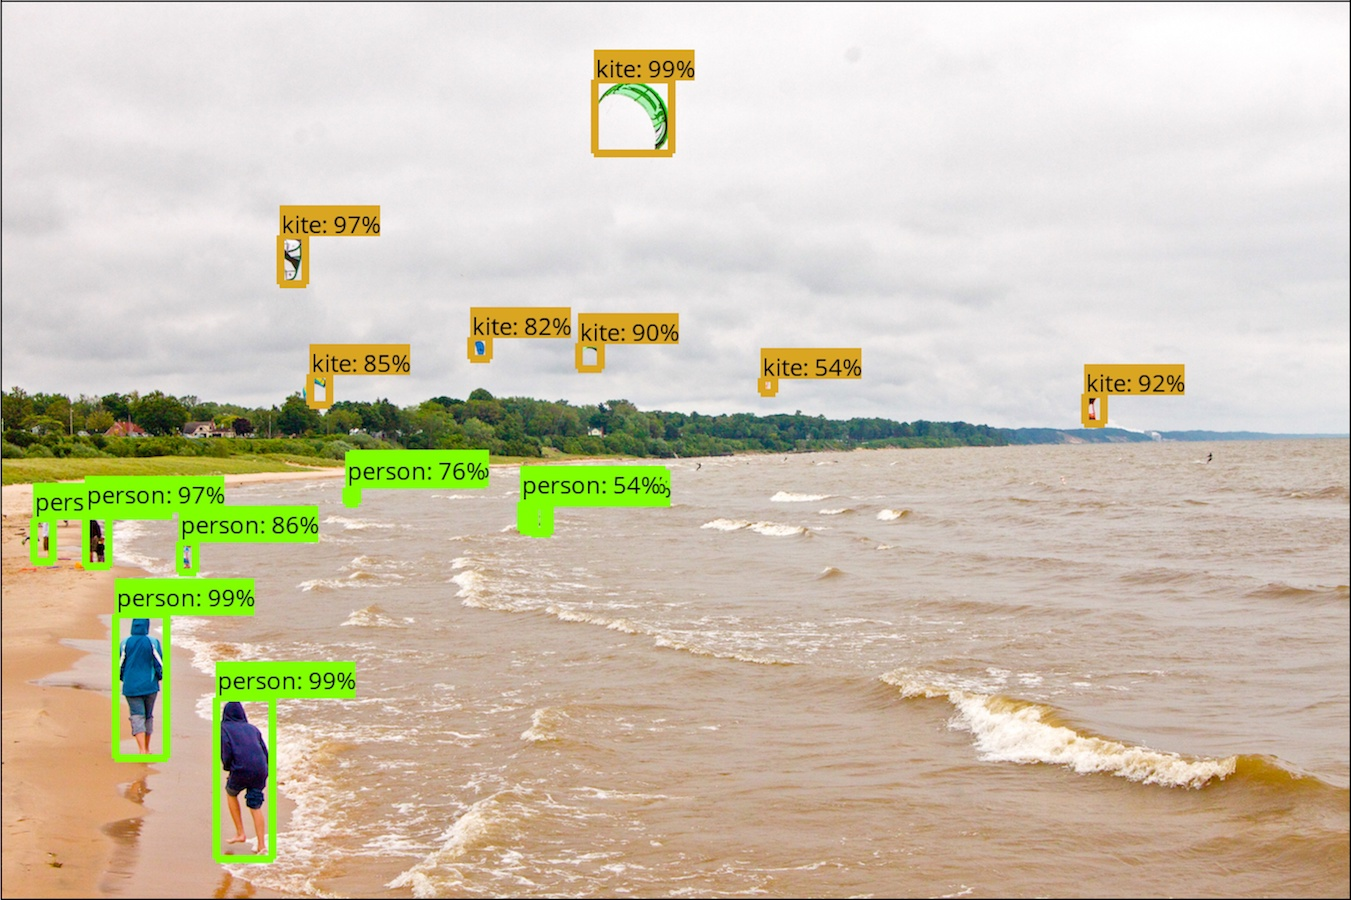
\includegraphics[width=0.60\textwidth]{img/objectdetection.jpg}
	\legend{Fonte: \citeonline{websiteObjectDetection}}
	\label{fig:objectdetection}
\end{figure}

Este trabalho consiste em criar um sistema de visão computacional capaz de detectar células em uma imagem, para assim realizar a contagem e posteriormente criar os elementos de um hemograma. Logo, o módulo de detecção de objetos se alinha com esse conceito. Embora seja normalmente utilizado para detecção de pessoas e objetos, este módulo possui grande capacidade de personalização, o que permite aprendizado voltado aos elementos que compõem o sangue. Ou seja, ao realizar o treinamento do modelo com base em um grande volume de imagens de sangue, é possível aprender com os dados para depois realizar as predições.

Como base para a utilização dessa biblioteca, a documentação foi de extrema importância para o entendimento dos seus recursos e limitações. No módulo de detecção de objetos, a documentação foi mais escassa, porém auxiliou em muitas questões do projeto, principalmente nos códigos base. Os primeiros códigos foram desenvolvidos com base nos exemplos de teste presentes na documentação, que permitiram ter uma grande noção das configurações possíveis de serem realizadas no modelo computacional e também de como é o funcionamento geral.

Para a execução dos códigos, porém, foi constatado que uma preparação do ambiente é necessária para atingir o melhor desempenho possível. Se fez necessário configurar corretamente a conexão do algoritmo para execução na placa de vídeo (GPU), ao invés de executar no processador (CPU) como é o padrão. Como o foco é trabalhar com processamento de imagens, ainda mais com um grande volume, as GPU's possuem um desempenho muito mais eficaz, entregando resultados melhores em menor tempo.

Para a preparação do ambiente, foi necessário primeiramente realizar a instalação do CUDA. O CUDA é uma plataforma da NVIDIA para realização de computação paralela, para fornecer aos desenvolvedores o melhor aproveitamento do processamento das placas de video e acelerar drasticamente os aplicativos de computação. Adicional ao CUDA, também é interessante o uso de uma biblioteca conhecida por cuDNN. O cuDNN é uma biblioteca com foco em \emph{Deep Neural Network}, ou seja, redes neurais profundas, que permite utilizar estruturas de redes neurais no trabalho com algoritmos de aprendizagem de máquina, sendo perfeitamente alinhado com o propósito desse trabalho. O uso do CUDA associado ao cuDNN, aumenta a eficiência e também a qualidade do resultado. \cite{websiteCUDA, websiteCUDNN}

Com a preparação do ambiente finalizada, o algoritmo já pode ser executado sem maiores problemas. Nessa etapa alguns testes foram realizados, executando os exemplos base presentes na documentação, para ter uma ideia de como o algoritmo se comporta na máquina e quais seriam os resultados do processamento de exemplo e em quanto tempo seriam entregues. Essa etapa foi importante para a continuidade dos trabalhos, pois foi possível ter uma noção de tempo necessário para execução dos códigos, permitindo aprimorar o planejamento das próximas etapas do projeto.

\section{Modelo Computacional}
Com todos os recursos, bibliotecas e ambiente funcionando em harmonia, iniciou-se o processo para inserir o \emph{dataset} nos moldes do modelo para o treinamento e reconhecimento das imagens. O conjunto de imagens estava adequadamente formatado para o uso pelo algoritmo, estando em um tamanho suficientemente bom, além de possuírem todas o mesmo tamanho e a mesma escala de ampliação.

Para o reconhecimento das coordenadas das imagens, primeiro, foi necessário a importação e tratamento dos arquivos XML em variáveis capazes de serem lidas pelo modelo. Contudo, apenas essa importação não foi o suficiente, visto que os dados contidos nos arquivos e os aceitos pelo modelo estavam em escalas e proporções diferentes. Ou seja, o algoritmo não estava conseguindo encontrar as células nas imagens durante a importação. Para adequar esse processo, foi necessário criar uma função capaz de converter as coordenadas do XML em números na escala do modelo, permitindo assim, importar tanto as coordenadas, quanto as imagens com sucesso.

Dessa forma, foi possível realizar um teste primário, sem alterar as características do modelo, para um dos tipos de células primeiramente, o que retornou resultados satisfatórios para essa condição. Porém para se obter um ganho total dos conceitos do modelo, foi necessário a realização de ajustes nas configurações dos seguintes atributos:

\begin{itemize}
    \item \emph{Batch Size}: Significa o tamanho do lote utilizado no treinamento. Geralmente quanto maior o lote, melhor o aprendizado, porém também é necessário mais processamento da máquina.
    \item \emph{Learning Rate}: Significa a taxa de aprendizado do modelo. Quanto maior, mais rápido os passos de aprendizado serão realizados. Caso seja muito grande, o modelo começa a reconhecer células onde não existem. Caso seja muito pequeno, o modelo não encontra nenhuma célula nas imagens.
    \item Número de \emph{Batches}: Significa o número de passadas do algoritmo, também pode ser descrito como épocas. Define o intervalo de execuções que o algoritmo terá até parar o treinamento.
    \item Porcentagem de Acerto: Significa o número base para ser considerado um acerto de fato, por exemplo, se o algoritmo tem mais de 50\% de certeza para uma célula, é considerado acerto.
\end{itemize}

Esses parâmetros foram configurados com base em testes realizados, onde a cada execução do código, foi verificado e ajustado conforme o necessário. Esse processo foi realizado até encontrar os valores mais adequados que retornam os melhores resultados. Os valores finais utilizados podem ser conferidos no capítulo \ref{chap:resultados}.

Além da configuração desses parâmetros, também existe outro ponto bastante importante e necessário para este trabalho, o qual consiste em selecionar uma rede neural pré-treinada adequada para o uso. Através de uma rede pré-treinada, muitos parâmetros comuns podem ser aproveitados, agilizando o processo de treinamento de novos modelos. Além disso, também é capaz de impactar nos resultados, pois se foi devidamente treinada com informações básicas, como contornos e elementos comuns, os resultados ao treinar com elementos mais complexos serão melhores.

Para este trabalho, foi selecionada a rede ``resnet50'', embora existam muitas outras incluídas na lista da documentação aceitas pelo módulo de detecção de objetos. Essa escolha foi definida pelo tamanho da imagem utilizada e também ao realizar testes de desempenho em comparação com as outras redes \cite{websiteObjectDetection}.

Com o treinamento de um tipo de célula realizado com sucesso, foi necessário expandir para treinar as demais. Primeiramente, foi testado treinando todas as células de uma só vez, porém essa abordagem estava consumindo muitos recursos da máquina e produzindo resultados insatisfatórios.

Nesse caso, a abordagem precisou ser alterada. Ao invés de treinar todos os tipos de células de uma só vez, foi criado um modelo único para cada uma delas, no caso um modelo para células brancas, outro para as vermelhas e um para as plaquetas. Isso permitiu que o treinamento fosse mais eficiente e com resultados mais assertivos e direcionados para cada tipo.

Como são utilizados 3 modelos, ao inserir uma imagem para verificação na predição de resultados, ela terá 3 respostas diferentes, sendo uma imagem de resultado para cada tipo de célula presente. Essa abordagem também permitiu utilizar valores de parâmetros diferentes para cada tipo, o que também auxiliou na melhora dos resultados para os diferentes tipos. Como o objetivo proposto neste trabalho é a contagem das células individuais, esta separação dos modelos para cada célula não tem influência negativa no resultado final.

\section{Avaliação}
Para a realização da avaliação, foram utilizadas métricas para medir o desempenho do modelo computacional e também para avaliar a qualidade dos resultados obtidos com cada um dos modelos treinados. As métricas foram utilizadas em cada uma das opções de modelos, utilizando configurações diferentes, para ter um comparativo entre uma opção e outra.

Dessa forma, foi possível avaliar e escolher com propriedade, qual algoritmo era o mais adequado para o uso no protótipo, assim como as melhores configurações possíveis para extrair o máximo desempenho da alternativa escolhida.

As métricas utilizadas para a avaliação, foram inicialmente a acurácia padrão para os primeiros testes. Posteriormente também foram medidas, utilizando o MSE (\emph{Mean Squared Error}), que significa erro quadrático médio e também foi estendido para o rMSE. o rMSE (\emph{Root Mean Squared Error}), sendo uma variação do MSE, onde é aplicada a raiz quadrada ao resultado.

A acurácia padrão foi a primeira métrica utilizada, sendo calculada considerando o número de células reais para serem encontradas pelo modelo e o número de células que o modelo realmente conseguiu encontrar. Com base na relação desses números também foi calculada a porcentagem geral de acurácia final.

O MSE, foi calculado com base na fórmula apresentada a seguir. Primeiramente, foi calculada a diferença entre o valor encontrado pelo modelo e o valor real de cada uma das imagens, para então calcular o quadrado do resultado obtido. Por fim, é realizada a média desses valores para todas as imagens, gerando erro quadrático médio.

\[ MSE = \frac{1}{n}\sum_{i=1}^{n} (\skew{4.5}\hat{y}_\iota - y_\iota)^{2} \]

O valor ideal desse número é perto de 0, pois quanto maior o número, maior o erro do modelo. Como o resultado é sempre elevado ao quadrado, predições distantes do real são facilmente perceptíveis, o que torna essa métrica interessante para problemas onde grandes erros não são tolerados.

O rMSE, foi calculado com base na fórmula apresentada abaixo. Como já foi calculado o MSE, foi possível calcular a raiz quadrada resultante para encontrar o rMSE final.

\[ rMSE = \sqrt{\frac{1}{n}\sum_{i=1}^{n} (\skew{4.5}\hat{y}_\iota - y_\iota)^{2}} \]

Essa métrica é um complemento do MSE normal, pois através dessa métrica, é possível mensurar de uma forma melhor a resultante final. Pois, enquanto o MSE está elevado o quadrado, o rMSE não tem esse problema, pois é extraída a raiz quadrada no processo final.

\section{Protótipo}
Após a definição da melhor instância do modelo computacional possível, seguindo as métricas definidas, foi realizada a exportação desse modelo, para então utilizá-lo na criação de um protótipo funcional.

Para realizar a exportação do modelo, a documentação da biblioteca do Tensorflow precisou ser analisada novamente, estudando de forma mais aprofundada o funcionamento dos \emph{checkpoints}. Os \emph{checkpoints} são uma estrutura presente no Tensorflow que permitem salvar o estado atual de um modelo treinado para ser utilizado posteriormente. Dessa forma, é possível utilizar um modelo pronto, sem precisar passar pelo processamento do treinamento novamente e sim, somente utilizá-lo para predições, com base em uma imagem de entrada. Sendo assim, o modelo pode ser usado em vários locais diferentes, apenas importando um arquivo \cite{websiteTensorFlow}.

Para a criação do protótipo, foi utilizada uma biblioteca com foco em prototipação de algoritmos de inteligência artificial, o Streamlit. O Streamlit é um framework para o uso em Python, que permite criar protótipos de uma forma fácil e rápida. É possível ter uma aplicação web com poucos comandos, permitindo focar no mais importante que é o código. Logo, não é necessário se preocupar com a parte da interface gráfica \cite{websiteStreamlit}.

Ainda assim é de fácil personalização, mostrando na tela todos os recursos do algoritmo, permitindo ao usuário enviar os dados de entrada (\emph{input}) e também conseguir visualizar o resultado recebido do algoritmo (\emph{output}). Dessa forma, é possível ter uma interação com o usuário em tempo real.

A Figura \ref{fig:prototipo} apresenta a interface do protótipo desenvolvido.

\begin{figure}[!htb]
	\centering
	\caption{Interface do protótipo desenvolvido.}
	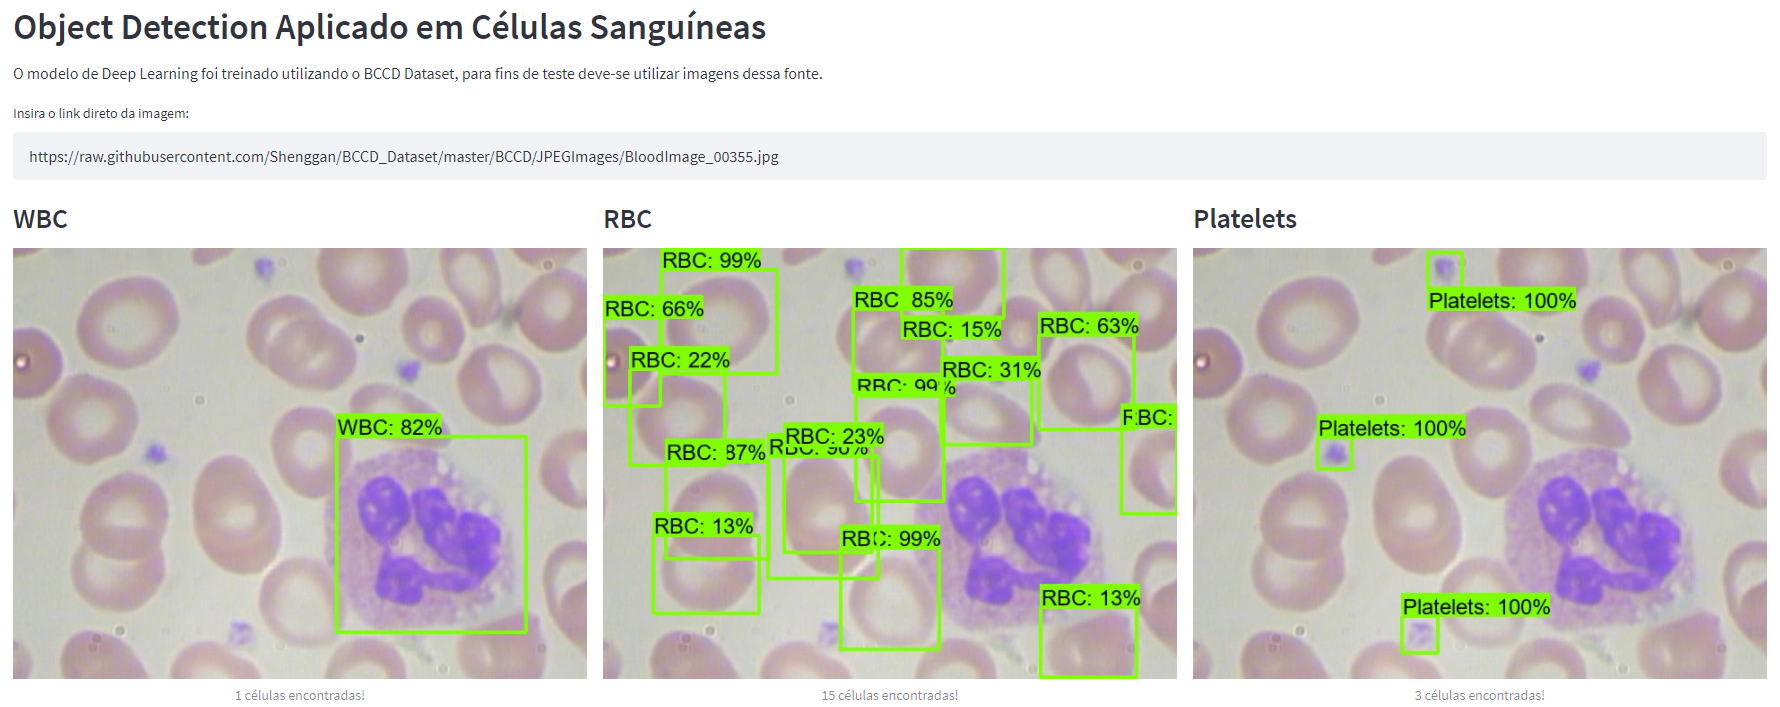
\includegraphics[width=1.0\textwidth]{img/prototipo.png}
	\legend{Fonte: Elaborado pelo autor.}
	\label{fig:prototipo}
\end{figure}

Como pode ser notado, o protótipo apresenta ao usuário um campo de entrada, onde é possível informar um \emph{link} de uma imagem da Internet, sendo recomendado o uso de imagens no formato do \emph{dataset} onde o modelo foi treinado. Na mesma Figura, também é possível visualizar um resultado do processamento de uma amostra de sangue, onde, nas imagens apresentadas, estão contidos o reconhecimento das células brancas, vermelhas e plaquetas, respectivamente, através no modelo treinado previamente.

\chapter{Resultados}
\label{chap:resultados}
Neste capítulo serão abordados todos os resultados do projeto desenvolvido, os quais foram todos avaliados através das métricas e conceitos apresentados no Capítulo anterior. Dessa forma, será apresentado em detalhes como os resultados foram obtidos, medidos e avaliados a partir das métricas, e também apresentadas imagens produzidas pelo modelo treinado. 

\section{Análise de Desempenho do Modelo}

O \emph{dataset} utilizado como base para a realização deste trabalho, possui 364 imagens diferentes de amostras de sangue. Cada imagem pode conter até 30 células de classes diferentes, localizadas em diferentes porções da imagem. As classes utilizadas nessa pesquisa são células vermelhas (RBC), células brancas (WBC) e também plaquetas (\emph{Platelets}), as quais são identificadas através de coordenadas que indicam a localização de cada célula na imagem, e ficam armazenadas em arquivos XML que acompanham o \emph{dataset} em questão.

Este \emph{dataset} foi separado em dois principais grupos. O primeiro grupo se refere ao conjunto de imagens voltados apenas para o treino, com 80\% das imagens totais, esse grupo contém 291 imagens selecionadas aleatoriamente. Enquanto o segundo grupo, voltado apenas para o teste, com 20\% das imagens totais, contém 73 imagens separadas para este fim. Como o grupo de treino precisa ser maior para se ter um bom treinamento do modelo e por fim realizar o teste nas imagens restantes, a seleção de 80/20 da separação dos arquivos foi adotada.

Como observado no Capítulo \ref{chap:metodologia}, o modelo foi configurado seguindo alguns princípios e configurações principais. Primeiramente foi selecionada a rede neural pré-treinada com o melhor resultado e performance para este grupo de imagem, sendo essa a ``resnet50'', reconhecida na base de código por ``ssd\_resnet50\_v1\_fpn\_640x640\_coco17\_tpu-8''. Além dessa escolha, quatro parâmtros fundamentais foram cuidadosamente selecionados, buscando o melhor desempenho em menor tempo. A definição dos parâmetros de \emph{Batch Size}, \emph{Learning Rate}, Número de \emph{Batches} e também a porcentagem de acerto base podem ser visualizados na Tabela \ref{tbl:parametros}.

\begin{table}[!htb]
\centering
\caption{Parâmetros Definidos}
\label{tbl:parametros}
\begin{tabular}{|c|c|c|c|}
\hline
                      & WBC  & RBC  & Platelets \\ \hline
Batch Size            & 24   & 24   & 24        \\ \hline
Learning Rate         & 0.02 & 0.05 & 0.05      \\ \hline
Número de Batches     & 500  & 500  & 500       \\ \hline
Porcentagem de Acerto & 0.5 & 0.1 & 0.5      \\ \hline
\end{tabular}
	\vspace{6pt}
	\legend{Fonte: Elaborada pelo autor.}
\end{table}

Após o treinamento do modelo, as predições foram medidas utilizando 3 métricas diferentes. A primeira foi a acurácia padrão, que permite ter uma visão geral do andamento do processo. Realizando a medição da acurácia padrão, considerando o número de células reais e o número de células que deveriam ser encontradas pelo modelo, se chegou na seguinte relação, utilizando o melhor resultado possível como parâmetro:

\begin{itemize}
    \item WBC: 74 células encontradas de 74 células reais (100,00\% de Acerto e 0,00\% de Falha)
    \item RBC: 1007 células encontradas de 908 células reais (89,10\% de Acerto e 10,90\% de Falha)
    \item Platelets: 57 células encontradas de 59 células reais (96,61\% de Acerto e 3,39\% de Falha)
\end{itemize}

Conforme constatado no Capítulo \ref{chap:metodologia}, o MSE e o rMSE, são métricas complementares, de fácil utilização e dizem muito a respeito do desempenho de um modelo computacional. Enquanto o MSE trabalha realizando o cálculo do erro quadrático médio, o rMSE é a raiz desse valor encontrado. Tais métricas são interessantes de se utilizar, pois, permitem visualizar de forma considerável, até mesmo pequenos erros. Essa escala não apresenta um número máximo ou ideal, mas o resultado deve se aproximar de zero, quanto mais próximo, melhor. Dessa forma, utilizando as fórmulas do capítulo anterior, foi possível chegar na relação da tabela \ref{tbl:mse}.

\begin{table}[!htb]
	\centering
	\caption{MSE e rMSE}
	\label{tbl:mse}
	\begin{tabular}{|c|c|c|}
		\hline
		          & MSE                & rMSE               \\ \hline
		WBC       & 0.3835616438356164 & 0.6193235372853323 \\ \hline
		RBC       & 14.342465753424657 & 3.787144802278447  \\ \hline
		Platelets & 0.9041095890410958 & 0.9508467747440151 \\ \hline
	\end{tabular}
	\vspace{6pt}
	\legend{Fonte: Elaborada pelo autor.}
\end{table}

Através da relação da Tabela \ref{tbl:mse}, foi possível perceber que o melhor desempenho está na detecção de células brancas, o que se alinha com as definições encontradas pela acurácia vista anteriormente. Isso pode ter acontecido, pois, no \emph{dataset}, em grande parte das imagens existe pelo menos uma célula branca que é facilmente detectada em relação às demais. Seguinte a isso, as plaquetas também apresentam bons resultados, parecido com a relação da acurácia do modelo. Por fim, as células vermelhas apresentam resultados inferiores em relação às demais. Isso pode ter acontecido, devido ao fato da sua abundância em todas as imagens, enquanto as outras classes apresentam uma ou duas células por imagem, as células vermelhas podem aparecer em um número maior que 20, isso dificulta o aprendizado do modelo e também atrapalha na predição nesse caso.

\section{Identificação de Células Brancas (WBC)}
A primeira classe de células trabalhadas, desde o primeiro teste utilizando o \emph{dataset} foram as células brancas. Isso ocorreu pela sua fácil identificação em relação as demais, sendo um ótimo candidato para se iniciar os testes e posteriormente as primeiras versões do protótipo.

Essas células estão presentes nas imagens em baixa quantidade, pois o \emph{dataset} buscou focalizar uma célula branca em cada imagem. Embora em alguns casos seja possível encontrar até duas ou três. Além da quantidade, podem ser diferenciadas das outras através da sua coloração.

\begin{figure}[!htb]
	\centering
	\caption{Detecção de Célula - WBC}
	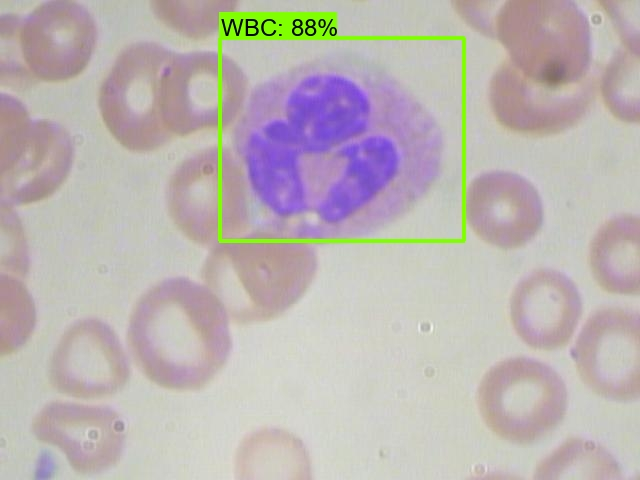
\includegraphics[width=0.60\textwidth]{img/predict_wbc.jpeg}
	\legend{Fonte: Elaborado pelo autor.}
	\label{fig:predict_wbc}
\end{figure}

Na Figura \ref{fig:predict_wbc} pode ser observado a detecção da célula branca pelo modelo. Onde foi possível diferenciar e delimitar a célula de forma bastante satisfatória. Na Figura \ref{fig:predict_wbc_2} também pode ser observado o mesmo processo, mas em outra situação.

\begin{figure}[!htb]
	\centering
	\caption{Detecção de Célula - WBC}
	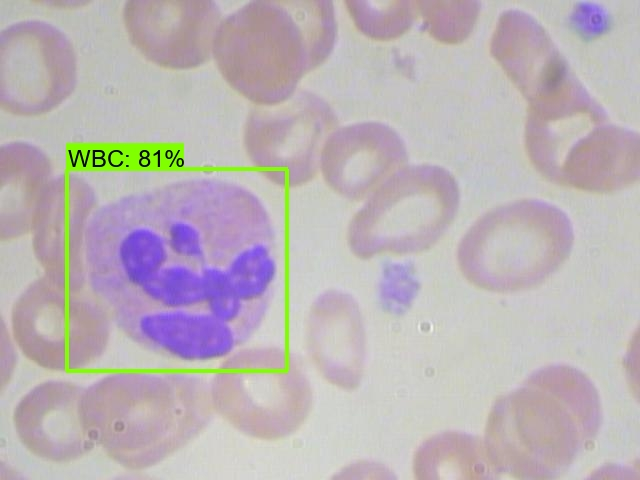
\includegraphics[width=0.60\textwidth]{img/predict_wbc_2.jpeg}
	\legend{Fonte: Elaborado pelo autor.}
	\label{fig:predict_wbc_2}
\end{figure}

Pôde-se perceber que o modelo obteve boa taxa de acerto, levando em consideração tanto as métricas de desempenho, quanto através da análise visual das imagens. Deste modo, é possível realizar as contagens das células com bom índice de assertividade.

\section{Identificação de Células Vermelhas (RBC)}
Após a detecção das células brancas, o próximo passo buscado foi a interpretação das células vermelhas. Essas se diferenciam na sua detecção em relação às outras devido a sua quantidade. As células vermelhas aparecem em uma proporção muito maior, constando até mesmo mais de 20 células por imagem.

A grande quantidade desse tipo de células é um desafio para o modelo, principalmente pela delimitação de suas áreas. Por não terem forma definida e muitas vezes se sobrepondo uma sobre as outras, isso atrapalha a sua identificação.

Na Figura \ref{fig:predict_rbc} podemos visualizar o processo de detecção das células vermelhas. Sendo possível realizar a contagem das células conforme o necessário, com uma pequena margem de erro. 

\begin{figure}[!htb]
	\centering
	\caption{Detecção de Células - RBC}
	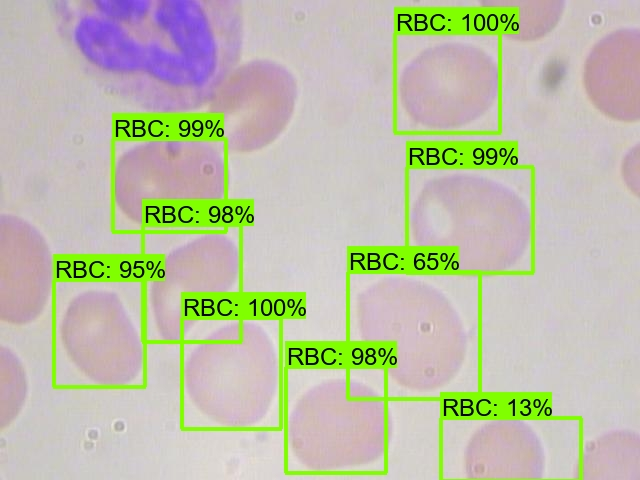
\includegraphics[width=0.60\textwidth]{img/predict_rbc.jpeg}
	\legend{Fonte: Elaborado pelo autor.}
	\label{fig:predict_rbc}
\end{figure}

Entretanto, na Figura \ref{fig:predict_rbc_2} também é possível visualizar a identificação pelo modelo, porém em uma densidade muito maior, mesmo com a sobreposição de células, ainda assim o modelo conseguiu identificar a maior parte das células de forma correta.

\begin{figure}[!htb]
	\centering
	\caption{Detecção de Células - RBC}
	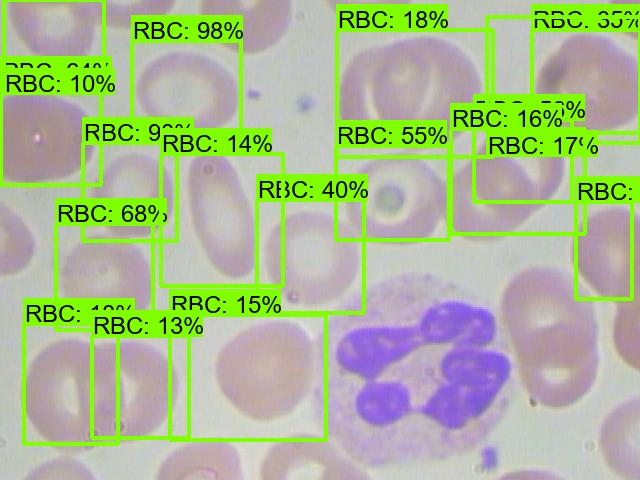
\includegraphics[width=0.60\textwidth]{img/predict_rbc_2.jpeg}
	\legend{Fonte: Elaborado pelo autor.}
	\label{fig:predict_rbc_2}
\end{figure}

É possível concluir que embora não tenha um desempenho tão positivo quanto as demais classes, os resultados também são bons pois permitem uma contagem das células vermelhas com uma pequena margem de erro.

\section{Identificação de Plaquetas (\emph{Platelets})}

Por fim, a detecção das plaquetas foram realizadas de forma similar as células brancas. Apesar de estarem mais presentes no \emph{dataset} do que as células brancas, elas não estão em um número tão elevado quanto as células vermelhas, apresentando pequenos conjuntos por imagens. Outro fator característico em relação as demais é o seu tamanho, que é muito menor e de fácil identificação a olho nu.

Embora sejam identificadas de forma mais tranquila, a sobreposição de células também pode acontecer nesse caso, atrapalhando o desempenho da identificação pelo modelo. Porém isso acontece em um número significantemente menor em comparação com as células vermelhas.

É possível visualizar na Figura \ref{fig:predict_platelets} o processo de identificação de células brancas, onde o modelo apresenta um desempenho considerado ótimo.

\begin{figure}[!htb]
	\centering
	\caption{Detecção de Células - Platelets}
	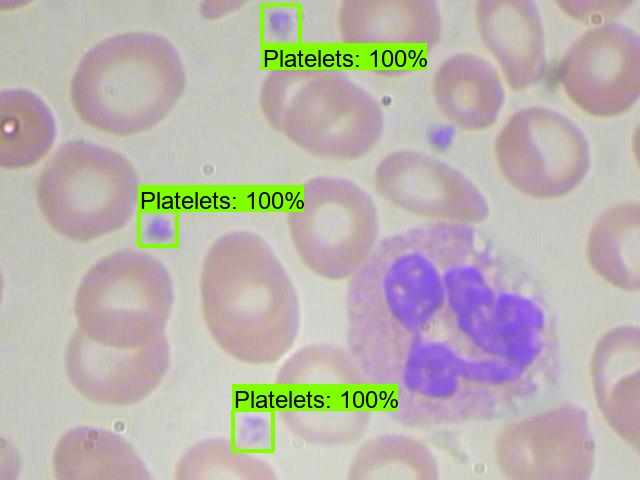
\includegraphics[width=0.60\textwidth]{img/predict_platelets.jpeg}
	\legend{Fonte: Elaborado pelo autor.}
	\label{fig:predict_platelets}
\end{figure}

Já na Figura \ref{fig:predict_platelets_2} é possível notar uma situação um pouco diferente. Nessa análise o modelo foi capaz de identificar corretamente as 4 plaquetas que aparecem na imagem, porém com margem de confiança do algoritmo levemente reduzida. 

\begin{figure}[!htb]
	\centering
	\caption{Detecção de Células - Platelets}
	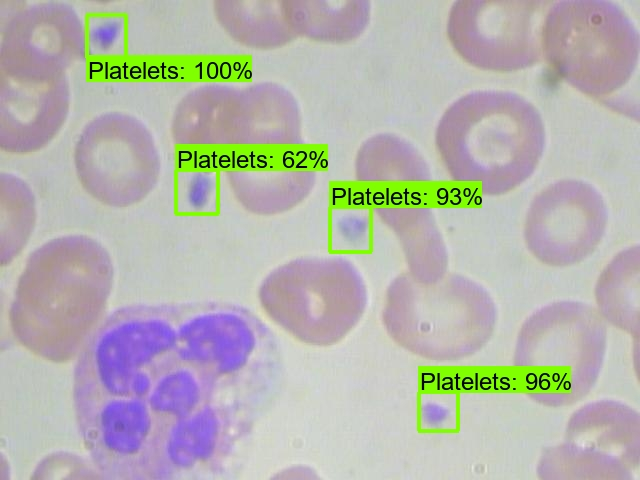
\includegraphics[width=0.60\textwidth]{img/predict_platelets_2.jpeg}
	\legend{Fonte: Elaborado pelo autor.}
	\label{fig:predict_platelets_2}
\end{figure}

Com isso, podemos concluir que as plaquetas possuem um desempenho adequado na sua identificação permitindo uma contagem satisfatória. Embora não seja tão positivo quando na detecção das células brancas, ainda supera as células vermelhas em relação ao desempenho e critérios de assertividade.

\section{Elaboração de Elementos do Hemograma}

Com base na identificação e na contagem das células, como visto anteriormente, é possível realizar a produção de um hemograma. Um hemograma é basicamente uma contagem das células e comparação desses resultados com índices pré-calculados de valores ideais para cada tipo de paciente.

Os valores iniciais do hemograma podem ser calculados realizando, após a identificação das células, a contagem de cada tipo. As unidades de medida são importantes nesse processo, pois são diferentes para cada tipo de célula. A unidade base para o cálculo é o milímetro cúbico (mm³), ou seja, uma unidade de volume. Para o cálculo dos leucócitos, que são as células brancas, e também das plaquetas é realizada a contagem em proporção a um milímetro cúbico. Porém, no caso dos eritrócitos, que são as células vermelhas, elas estão em uma quantidade muito maior em relação às outras células, portanto é realizado o cálculo de milhões de células em um milímetro cúbico.

O eritrograma pode ser elaborado, considerando o número de eritrócitos em uma relação de milhões/mm³. O leucograma pode ser elaborado, utilizando o número de leucócitos encontrados em unidade/mm³. E por fim o plaquetograma pode ser elaborado, com base no número de plaquetas identificadas em unidades/mm³.

Desta forma, com esse hemograma parcial várias doenças e desequilíbrios do organismo do paciente podem ser identificados. Como por exemplo, o leucograma sendo o principal exame para avaliar a imunidade de uma pessoa, através da quantidade de leucócitos presentes no organismo. O número das plaquetas também muito diz sobre o organismo, avaliando a coagulação sangúinea do indivíduo e pré-disposições à hemorragias. Assim como, o número de hemácias baixo, poderia indicar uma anemia ou doença associada, entre muitos outros casos.

Podemos concluir que através desses dados, é possível elaborar um hemograma parcial bastante útil e interessante para o uso. Caso os valores de um exame como este estejam alterados e fora do padrão considerado aceito mundialmente. Nesse caso seria necessário realizar uma investigação mais aprofundada com exames mais específicos a cada situação.

As limitações para a elaboração de um hemograma total estão relacionadas com as limitações do \emph{dataset}. Primeiramente, para a realização de um hemograma completo, seria necessário ter além da contagem, também a classificação das células brancas. Sua classificação em Monócitos, Leucócitos, Neutrófilos, Eosinófilos, Basófilos, Linfócitos, entre outros é necessária para a completude do exame. Porém, essas classificações não são apresentadas pelo \emph{dataset}, que procura focar apenas nas diferenciações entre os três principais tipos.

Outros valores relacionados à cálculos com volume, como o VCM (Volume Corpuscular Médio) e também o HCM (Hemoglobina Corpuscular Média), entre os outros citados no Capítulo \ref{chap:fund} não são possíveis de serem calculados por falta de informação. Na utilização de outro \emph{dataset} em trabalhos futuros, essas informações podem ser calculadas tranquilamente a partir da coleta de dados, como será abordado no próximo capítulo. 
